\documentclass[
	a4paper,
	oneside,
	DIV = 12,
	fontsize = 13pt,
	headings = normal,
]{scrartcl}

%%% Page geometry and precise margins
\usepackage[
	pass,
	left   = 20mm,
	top    = 15mm,
	right  = 10mm,
	bottom = 15mm,
]{geometry}
%%%

%%% Length calculations
\usepackage{calc}
%%%

%%% Support for color
\usepackage{xcolor}
\definecolor{lightblue}{HTML}{03A9F4}
\definecolor{red}{HTML}{F44336}
%%%

%%% Including graphics
\usepackage{graphicx}
%%%

%%% Font selection
\usepackage{fontspec}

\setromanfont{STIX Two Text}[
	SmallCapsFeatures = {LetterSpace = 5},
]

\setsansfont{IBM Plex Sans}[
	Scale = MatchUppercase,
]

\setmonofont{IBM Plex Mono}[
	Scale = MatchUppercase,
]
%%%

%%% Math typesetting
\usepackage{amsmath}

\usepackage{unicode-math}
\setmathfont{STIX Two Math}
%%%

%%% List settings
\usepackage{enumitem}
\setlist[enumerate]{
	label*      = {\arabic*.},
	leftmargin  = *,
	labelindent = \parindent,
	topsep      = 1\baselineskip,
	parsep      = 0\baselineskip,
	itemsep     = 1\baselineskip,
}

\setlist[itemize]{
	label       = {—},
	leftmargin  = *,
	labelindent = \parindent,
	topsep      = 1\baselineskip,
	parsep      = 0\baselineskip,
	itemsep     = 1\baselineskip,
}

\setlist[description]{
	font        = {\rmfamily\upshape\bfseries},
	topsep      = 1\baselineskip,
	parsep      = 0\baselineskip,
	itemsep     = 0\baselineskip,
}

%%%

%%% Structural elements typesetting
\setkomafont{pagenumber}{\rmfamily}
\setkomafont{disposition}{\rmfamily\bfseries}

% Sectioning
\RedeclareSectionCommand[
	beforeskip = -1\baselineskip,
	afterskip  = 1\baselineskip,
	font       = {\normalsize\bfseries\scshape},
]{section}

\RedeclareSectionCommand[
	beforeskip = -1\baselineskip,
	afterskip  = 1\baselineskip,
	font       = {\normalsize\bfseries},
]{subsection}

\RedeclareSectionCommand[
	beforeskip = -1\baselineskip,
	afterskip  = 1\baselineskip,
	font       = {\normalsize\bfseries},
]{subsubsection}
%%%

%%% Typographic enhancements
\usepackage{microtype}
%%%

%%% Language-specific settings
\usepackage{polyglossia}
\setmainlanguage{ukrainian}
\setotherlanguages{english, russian}
%%%

%%% Captions
\usepackage{caption}
\usepackage{subcaption}

%\DeclareCaptionLabelFormat{closing}{#2)}
%\captionsetup[subtable]{labelformat = closing}

%\captionsetup[subfigure]{labelformat = closing}

\captionsetup[table]{
	aboveskip = 0\baselineskip,
	belowskip = 1\baselineskip,
}

\captionsetup[figure]{
	aboveskip = 1\baselineskip,
	belowskip = 0\baselineskip,
}

\captionsetup[subfigure]{
	aboveskip = 0.25\baselineskip,
	belowskip = 0\baselineskip,
}

\captionsetup[subfigure]{
	labelformat = simple,
	labelformat = brace,
}
%%%

%%% Table typesetting
\usepackage{booktabs}
\usepackage{longtable}

\usepackage{multirow}

\usepackage{array}
\newcolumntype{v}[1]{>{\raggedright\arraybackslash\hspace{0pt}}p{#1}}
\newcolumntype{b}[1]{>{\centering\arraybackslash\hspace{0pt}}p{#1}}
\newcolumntype{n}[1]{>{\raggedleft\arraybackslash\hspace{0pt}}p{#1}}
%%%

%%% Dingbats
\usepackage{pifont}
%%%

%%% TikZ
\usepackage{tikz}
%%%

%%% Links and hyperreferences
\usepackage{hyperref}
\hypersetup{
	bookmarksnumbered = true,
	colorlinks      = false,
	linkbordercolor = red,
	urlbordercolor  = lightblue,
	pdfborderstyle  = {/S/U/W 1.5},
}
%%%

%%% Length adjustments
% Set baselineskip to ~15pt, default is 14.5pt
% \linespread{1.034483}
% \linespread{1.068966} % ~15.5pt
\setlength{\emergencystretch}{1em}
\setlength{\parindent}{1.5em}
\newlength{\gridunitwidth}
\setlength{\gridunitwidth}{\textwidth / 12}
\setlength{\floatsep}{1\baselineskip}
\setlength{\intextsep}{1\baselineskip}
\setlength{\textfloatsep}{1\baselineskip}
%%%

%%% Custom commands
\newcommand{\allcaps}[1]{{\addfontfeatures{LetterSpace = 5}#1}}
\newcommand{\progname}[1]{\texttt{#1}}

\newcommand{\CheckMark}{\ding{51}}
\newcommand{\Mytextrightarrow}{$\rightarrow$\hspace{0.25em}}
%%%

%%% Make typography adhere to made-up standards
\PolyglossiaSetup{ukrainian}{indentfirst = true}

% Sectioning
\RedeclareSectionCommand[
	beforeskip = -0.75\baselineskip,
	afterskip  = 0.25\baselineskip,
	indent     = 12.5mm,
	font       = {\normalsize\bfseries},
]{section}

\RedeclareSectionCommand[
	beforeskip = -0.75\baselineskip,
	afterskip  = 0.25\baselineskip,
	indent     = 12.5mm,
	font       = {\normalsize\bfseries},
]{subsection}

\RedeclareSectionCommand[
	beforeskip = -0.75\baselineskip,
	afterskip  = 0.25\baselineskip,
	indent     = 12.5mm,
	font       = {\normalsize\bfseries},
]{subsubsection}

\setlength{\parindent}{12.5mm}

\usepackage{leading}
\leading{21pt}

%%%

\begin{document}
	\newgeometry{
		left   = 20mm,
		top    = 15mm,
		right  = 10mm,
		bottom = 15mm,
		footskip = \baselineskip, % reduce footer vertical skip so page numbers are visible
	}
\setlength{\gridunitwidth}{\textwidth / 12}
	\begin{titlepage}
		\begin{center}
			Міністерство освіти і науки України\\
			Національний авіаційний університет\\
			Навчально-науковий інститут комп'ютерних інформаційних технологій\\
			Кафедра комп'ютеризованих систем управління

			\vspace{\fill}
				Лабораторна робота №3\\
				з~дисципліни «Діагностика та~експлуатація комп'ютера»\\
				на~тему «Відновлення даних на~жорсткому диску»\\

			\vspace{\fill}

			\begin{flushright}
				Виконав:\\
				студент \allcaps{ННІКІТ}\\
				групи СП-325\\
				Клокун В.\,Д.\\
				Перевірив:\\
				Масловський Б.\,Г.
			\end{flushright}

			Київ 2018
		\end{center}
	\end{titlepage}

	\section{Ціль роботи}
		Ознайомлення з~методами відновлення даних на~жорсткому диску.

	\section{Короткі теоретичні відомості}
		Пошкодження даних може виникнути як~через помилки при~обробці таблиці файлів. Це може трапитися, наприклад, після некоректного відключення пристрою, збоїв в~роботі програмного і~апаратного забезпечення або в~результаті зараження вірусами. Також однією з~поширених причин виникнення такого роду помилок є~частковий вихід з~ладу поверхні диска~— поява «bad-секторів». На~жаль, зараз це~явище не~рідкість навіть для~нових жорстких дисків, що~експлуатуються протягом декількох тижнів або~навіть днів. 

		Якщо запис в~сектори, що~містять файли не~проводилася, то~дані фізично залишилися на~своїх місцях, але~загубилися або~спотворилися відомості про~їх~розташування. Таким чином, потрібно визначити, де~саме знаходяться сектора, містять потрібну інформацію, і~зчитати~їх у~правильній послідовності. 

		У~разі, коли проводився запис на~диск, наприклад, під час форматування диску з~подальшою установкою операційної системи, ймовірність фізичного знищення потрібної інформації може бути досить велика. У~подібних ситуаціях можливість успішного відновлення даних залежить від~везіння і~співвідношення обсягів втраченої і~записаної інформації. Скажімо, якщо Ви випадково видалили 1~Гб бухгалтерських баз і~після цього записали на~цей~же логічний розділ 70~Гб цікавих фільмів, ймовірність відновлення хоч чогось близька до~нуля. 

		Також варто взяти до~відома, що при~втраті даних через помилки в~файловій системі, запуск програм типу \textenglish{ScanDisk} істотно зменшує ймовірність успішного відновлення. Основне завдання цих утиліт~— приведення в~порядок службових структур файлової системи, що~вони і~роблять, не~особливо піклуючись про~долю користувача даних. При~цьому знищуються дані, за~якими можна було~б реконструювати структуру файлової системи до~пошкодження і~врятувати дані. 

		У~загальному випадку, програма для~відновлення даних спочатку сканує всі носії. За~результатами сканування, на~основі виявлених службових записів, складається карта розташування фрагментів відновлюваних файлів і~будується дерево каталогів. У~карті містяться відомості про~те, який кластер до~якогось файлу відноситься, розміри, назви та~інші атрибути елементів файлової системи, що~сканується, тобто все, що~вдалося дізнатися на~підставі залишків службової інформації. Якщо отриманих в~результаті сканування відомостей не~достатньо, то~використовуються певні методи екстраполяції. Потім файли і~папки, які~потрібно відновити, вибираються відповідно до~складеної карти і~переносяться на~інший носій. 

		Найчастіше все, що~в~принципі можливо відновити за~справного носія інформації, дістається за~допомогою програм, згаданих нижче. І~лише в~меншій частині випадків, висококваліфікований фахівець, працюючи на~більш низькому рівні, здатний відновити інформацію в~більшому обсязі. 

		Перед тим, як~приступити до~самостійного відновлення даних, слід взяти до~уваги можливість фізичної несправності пристрою. Особливо це~ймовірно у~випадках, коли дані пропали без~видимих причин, або~при~спробі відкриття файлів видається повідомлення про~помилку. І~хоча нижчезгаданих програми самі по~собі не~роблять деструктивних дій (вони взагалі нічого не~пишуть на~розділ, з~яким працюють), подальша робота з~несправним накопичувачем без~спеціального обладнання може привести до~посилювання ситуації, аж~до~повної неможливості відновлення даних. 

		Значний досвід використання різних програм для~відновлення даних показує, що~жодна з~них не~дає кращий результат у~всіх випадках втрати інформації. Вони використовують різні алгоритми, які~мають свої переваги і~недоліки. Тому, в~залежності від~характеру пошкодження, на~одній і~тій~же файлової системі кращий результат можуть показати різні утиліти. 

		Цей факт добре відомий, тому в~процесі роботи фахівцями використовуються добірки програм від~різних виробників, і~в~кожній ситуації застосовується утиліта, найкращим чином підходить під~конкретний випадок. Або~використовується декілька різних програм послідовно. 

		\textenglish{\allcaps{UFS} Explorer}~— найбільш універсальний з~відомих пакетів програм для~відновлення даних. \textenglish{UFS Explorer Standard Recovery} зручний для~професіоналів, підтримує відновлення інформації з~різних типів накопичувачів і~всіх поширених на~даний момент файлових систем. Є~версії під~\textenglish{Windows, Linux, \allcaps{BSD}, Mac~OS}. Редакція \textenglish{Raise Data Recovery} являє собою набір утиліт для~користувачів, яким потрібне разове відновлення даних. Функціонал кожної з~них обмежений підтримкою однієї конкретної файлової системи, працюють тільки під~\textenglish{Windows}. 

		Безкоштовна програма для відновлення даних \textenglish{R.saver} допоможе врятувати дані з~\textenglish{\allcaps{FAT}} або~\textenglish{\allcaps{NTFS}}. Вона призначена для~користувачів, не~знайомих з~пристроєм файлових систем і~принципами відновлення даних, тому інтерфейс максимально спрощений. Налаштування виконуються автоматично, для~запуску сканування достатньо натиснути всього одну кнопку. Це~робить програму менш зручною для~професіоналів, але~значно спрощує її~застосування звичайними користувачами. 

		Якщо алгоритми зазначених вище програм виявилися не~оптимальними для~конкретного випадку, рекомендується спробувати \textenglish{R-studio} або~\textenglish{GetDataBack}. 

		Послідовність дій при відновленні даних:
		\begin{enumerate}
			\item Встановлення або~розпакування завантаженої програми. Перш ніж приступити до~цих дій, переконайтеся, що~плануєте виконувати~їх на~диску або~розділі відмінному від~того, де~втрачена інформація. 

			\item Запуск і~попереднє сканування, яке~виконується автоматично. Утиліти використовують для~цього різні алгоритми, через~що у~них відрізняються час запуску і~списки виявлених файлових систем. Деякі програми можуть відразу показати пошкоджені розділи, які~не~видно засобами операційної системи, а~деякі не~покажуть навіть пристрій, з~якого планується відновити дані. Якщо все, що~потрібно, відобразилося, то~переходите до~третього пункту. Якщо~ні, то~можливі наступні варіанти: 
				\begin{itemize}
					\item	Пристрій відображається у~списку, але~потрібний розділ на~ньому не~знайдений: 
						\begin{itemize}
							\item Якщо такий функціонал програмою підтримується, то~можна скористатися поглибленим варіантом первинного сканування. Наприклад, в~\textenglish{\allcaps{UFS} Explorer} для~цієї мети є~функція «Знайти розділ». 

							\item Запустити сканування по~всьому пристрою відразу. Деякі програми, наприклад \textenglish{R-studio}, дозволяють це~зробити, показуючи в~результатах сканування можливі знайдені розділи з~приблизною файловими структурами. 

							\item Скористатися іншою програмою. 
						\end{itemize}

					\item	Пристрою немає у~списку, але~при~цьому визначається засобами операційної системи. В~\textenglish{Windows} це~можна перевірити, подивившись список пристроїв \textrussian{Пуск~\Mytextrightarrow Панель управления~\Mytextrightarrow Администрирование~\Mytextrightarrow Управление компьютером~\Mytextrightarrow Управление дисками}. Якщо накопичувач був підключений після запуску програми, то~перезапустіть~її або~поновіть список пристроїв. Якщо не~допомогло~— спробуйте іншу програму. 

					\item	Пристрій не~визначається засобами операційної системи. Перевірте правильність підключення і~подачу живлення. Якщо все підключено вірно, а~накопичувач все одно в~системі не~видно, то, найімовірніше, ви зіткнулися з~фізичною несправністю.
				\end{itemize}

			\item Налаштування параметрів сканування зазвичай виконується після вибору накопичувача або~розділу і~натиснення кнопки запуску, безпосередньо перед початком самого процесу. Деякі програми, в~тому числі \textenglish{R.saver}, виконують попереднє налаштування автоматично. Утиліта може запросити: 
				\begin{itemize}
					\item	Межі сканування. Якщо відомо, в~якій саме області пам'яті слід шукати потрібні дані, то~налаштування цих параметрів може заощадити час. Якщо не~знаєте~— залиште значення за~замовчуванням. 

					\item	Тип файлової системи. Деякі програми пропонують вибрати один тип зі~списку, підказуючи при~цьому оптимальний вибір, інші можуть запропонувати виключити зі~списку файлові системи, яких на~накопичувачі точно не~може бути. 

					\item	Для~певних типів файлових систем багатомовна програма може запросити передбачувану кодування. Наприклад, для~російськомовної \textenglish{\allcaps{FAT32}} слід вибирати \textenglish{cp866}. 

					\item	Крім перерахованих вище налаштувань, утиліти часто пропонують вибрати один або~кілька алгоритмів, які~будуть використовуватися в~процесі сканування. Їх~можна умовно розділити на~три типи, в~залежності від~призначення і~особливостей роботи: 
						\begin{itemize}
							\item Відновлення видалених файлів на~справній файловій системі. Повне сканування для~більшості типів файлових систем в~таких випадках не~потрібно. Використовується виключно для~відновлення видалених файлів. Деякі програми запускають його автоматично, в~процесі попереднього сканування. 

							\item Реконструкція файлової системи після пошкоджень або~форматування. Мета~— створення віртуального дерева каталогів, що~відображає вміст файлової системи, що~була сканована в~вихідному стані, без~пошкоджень. В~випадку успіху звідти можна зберегти потрібні дані на~інший розділ. 

							\item Відновлення даних по~сигнатурам, так зване «Чорнове» відновлення або~«Raw recovery». Сигнатура~— це~характерна послідовність символів, по~якої можна зрозуміти, що~знайдений фрагмент даних відноситься до~файлу певного типу. Використовується в~тих випадках, коли інші методи не~допомогли. Результатом застосування будуть файли без~назв, розсортовані по~папкам в~залежності від~типу містяться в~них даних. 
						\end{itemize}
				\end{itemize}

				Кожен тип носія інформації, файлова система і~особливості експлуатації, вносять свої критерії у~вибір оптимального методу відновлення даних. Наприклад, не~дивлячись на~те, що~відновлення по~сигнатурам рекомендується використовувати як~крайній захід, в~одному з~найпоширеніших випадків втрати даних його можна запустити відразу і~отримати відмінні результати. Цей~випадок~— випадкове видалення, форматування або~пошкодження структури \textenglish{\allcaps{FAT}}-флешки фотоапарата. Імена файлів і~структура папок в~таких випадках не~важливі. Крім того, фотографії звичайно пишуться послідовно на~порожню флешку, тому дані кожного файлу зберігаються разом у~вигляді одного ланцюжка. Це і~створює ідеальні умови для~використання «чорнового» відновлення. 

			\item Сканування може займати від~декількох хвилин до~декількох годин і~більше в~залежності від~характеристик накопичувача, способу його підключення до~комп'ютера і~використовуваних алгоритмів. Після завершення процесу утиліта відобразить вміст віртуальних каталогів із~знайденими файлами. 

			\item Вивчення результату сканування, вибір файлів для~збереження. У~багатьох програмах для~оцінки стану знайдених файлів передбачена функція попереднього перегляду. Потрібні файли помічаємо або~виділяємо. Якщо в~процесі перевірки частину шуканих даних виявити не~вдалося, саме час скористатися відновленням по~сигнатурам, якщо~це ще~не~було зроблено. 

			\item Збереження файлів~— по~суті це~і~є~саме відновлення даних, оскільки в~процесі сканування програма просто визначає розташування їх~фрагментів. Натискаємо відповідну кнопку на~панелі інструментів або~вибираємо розділ в~випадаючому меню. Потім вибираємо місце для~збереження. Переконайтеся, що~папка, в~яку буде зберігатися результат, знаходиться на~розділі або~носіях відмінному від~того, який сканувався. Далі тиснемо підтвердження і~очікуємо на~відновлені дані. 

		Перед закриттям програми переконайтеся, що~коректно відновилося все, що~потрібно, або~збережіть результат сканування. Інакше, якщо виявиться, що~вам потрібно щось~ще, доведеться сканувати заново. Це~може погіршити результат в~тих випадках, коли поверхня жорсткого диска починає виходити з~ладу. 

	\item Помилки читання, «зависання» програм під~час сканування жорсткого диска або~збереження результату можуть означати наявність секторів, що~не~читаються. Цілком імовірно, втрата даних і~була викликана їх~появою. Чим їх~більше, тим повільніше буде йти процес. Для перевірки припущення, можна скористатися \textenglish{HDDScan}. 
		\end{enumerate}

		У подібних випадках рекомендується зняти посекторну копію на~справний накопичувач і~відновлювати дані з~неї. Пам'ятайте, робота з~подібним диском погіршує його стан. Якщо не~впевнені в~тому, що~робите, і~на~диску важлива інформація~— краще зверніться в~спеціалізовану організацію. Там при~відновленні даних з~пошкоджених дисків використовують програмно-апаратні комплекси, спеціально призначені для~таких робіт.

	\section{Хід роботи}
		% Запускаємо \textenglish{VMware Player} та~додаємо новий жорсткий диск у~віртуальній машині. Для~цього заходимо у~налаштування віртуальної машини, натискаємо клавішу \textenglish{«Add…»}, обираємо тип апаратного забезпечення \textenglish{Hard Disk}, та~створюємо жорсткий диск типу~\textenglish{\allcaps{IDE}} розміром~5~Гб з~негайним виділенням та~зберіганням в~одному файлі. Запускаємо віртуальну машину з~встановленою операційною системою \textenglish{Windows~XP}.
		Запускаємо \textenglish{VMware Player} та~додаємо новий жорсткий диск у~віртуальній машині. Для~цього заходимо у~налаштування віртуальної машини, натискаємо клавішу \textenglish{«Add…»}, обираємо тип апаратного забезпечення \textenglish{Hard Disk}, обираємо тип диску \textenglish{\allcaps{IDE}}, встановлюємо, що для~додавання жорсткого диску його необхідно створити, задаємо розмір диску 5~Гб з~негайним виділенням та~зберіганням в~єдиному файлі, даємо цільовому диску назву та~натискаємо кнопку~\textenglish{«Finish»}. Запускаємо віртуальну машину з~встановленою операційною системою \textenglish{Windows~XP}.

		Створивши новий жорсткий диск, ініціалізуємо його в~операційній системі. Для цього відкриваємо утиліту «Управління дисками», яка~знаходиться за~шляхом \textenglish{Control Panel \Mytextrightarrow Administrative Tools \Mytextrightarrow Computer Management \Mytextrightarrow Storage \Mytextrightarrow Disk Management}.

		Ініціалізувавши диск в~операційній системі, створюємо тестові файли типів \textenglish{\allcaps{DLL}, \allcaps{JPG}} та~\textenglish{\allcaps{WMA}} і розміщуємо їх у спеціально відведеній директорії~(рис.~\ref{fig:01-created-files}). 

		\begin{figure}
			\centering
			\begin{subfigure}{0.5\columnwidth}
				\centering
				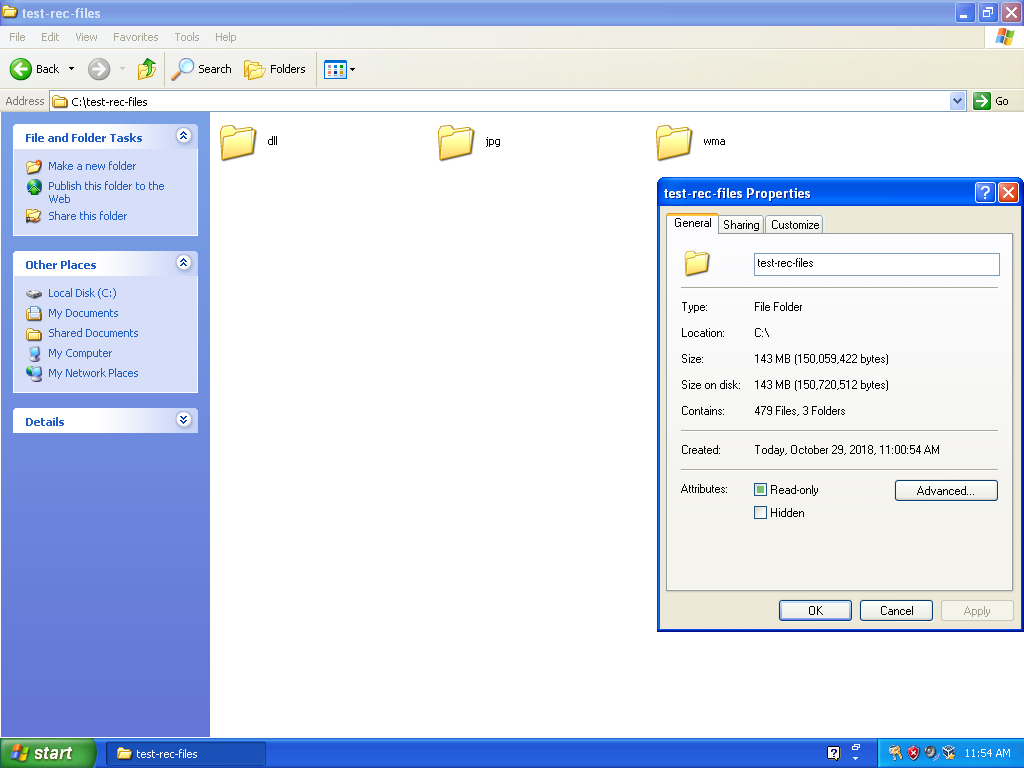
\includegraphics[height = 9\baselineskip]{./assets/y03s01-pcdiag-lab-03-p01.png}
				\caption{}
				\label{subfig:01-01-root}
			\end{subfigure}%
			\begin{subfigure}{0.5\columnwidth}
				\centering
				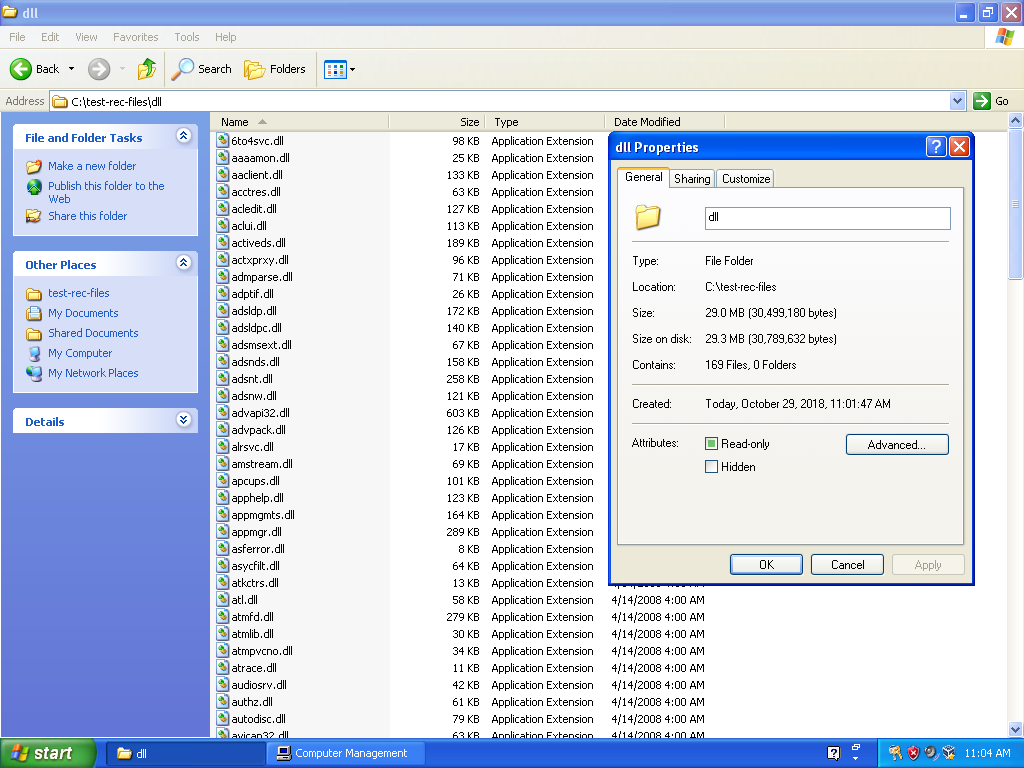
\includegraphics[height = 9\baselineskip]{./assets/y03s01-pcdiag-lab-03-p02.png}
				\caption{}
				\label{subfig:01-02-jpg}
			\end{subfigure}
			%
			\begin{subfigure}{0.5\columnwidth}
				\centering
				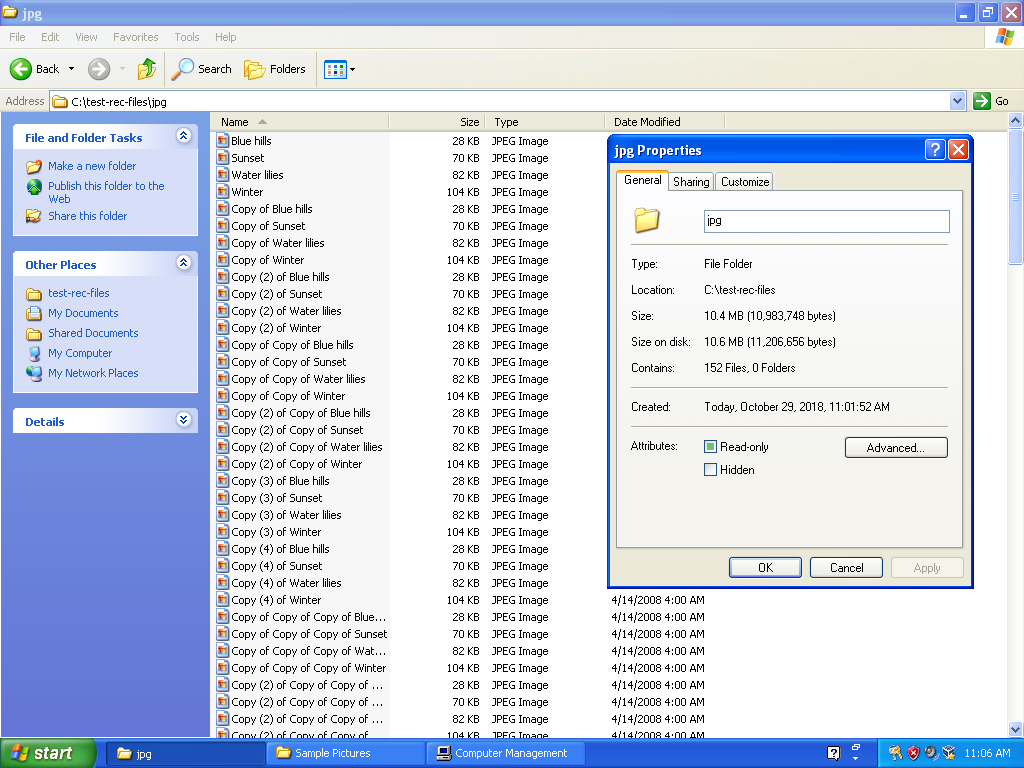
\includegraphics[height = 9\baselineskip]{./assets/y03s01-pcdiag-lab-03-p03.png}
				\caption{}
				\label{subfig:01-03-dll}
			\end{subfigure}%
			\begin{subfigure}{0.5\columnwidth}
				\centering
				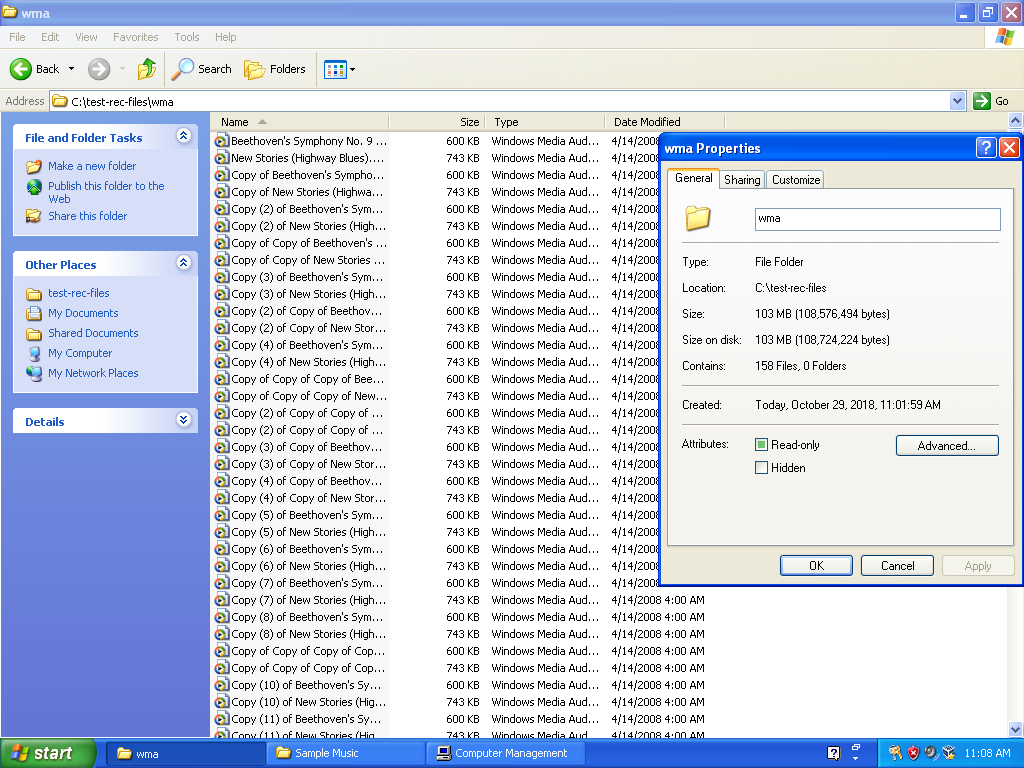
\includegraphics[height = 9\baselineskip]{./assets/y03s01-pcdiag-lab-03-p04.png}
				\caption{}
				\label{subfig:01-04-wav}
			\end{subfigure}%
			\caption{Вміст директорій зі створеними файлами: \subref{subfig:01-01-root}~— корінь, \subref{subfig:01-02-jpg}–\subref{subfig:01-04-wav}~— за типами файлів}
			\label{fig:01-created-files}
		\end{figure}

		Створивши необхідні файли, монтуємо диск з програмами \textenglish{R-Studio, Zero Assumption Recovery} та~встановлюємо їх. Після встановлення програм переходимо в~тестову директорію, переміщуємо туди створені файли та~видаляємо їх.

		Запускаємо програму \textenglish{R-Studio}, обираємо директорію, зміст якої необхідно відновити, та запускаємо процес~(рис.~\ref{fig:02-rstudio-recovery}). Після закінчення процесу відновлення отримали результат: 117~файлів з~479 початкових були успішно відновлені~(рис.~\ref{fig:03-rstudio-recovery-res}).

		 \begin{figure}[!htbp]
		 	\centering
		 	\begin{subfigure}{0.5\columnwidth}
		 		\centering
		 		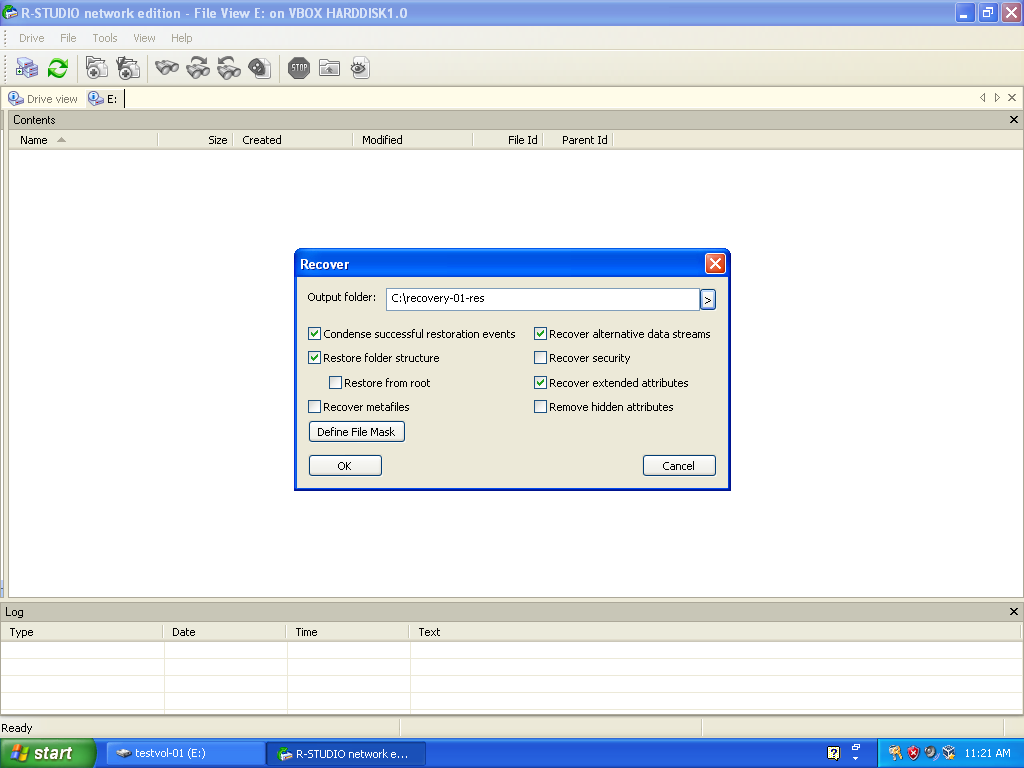
\includegraphics[height = 9\baselineskip]{./assets/y03s01-pcdiag-lab-03-p05.png}
		 		\caption{}
		 		\label{subfig:02-01-rstudio-start}
		 	\end{subfigure}%
		 	\begin{subfigure}{0.5\columnwidth}
		 		\centering
		 		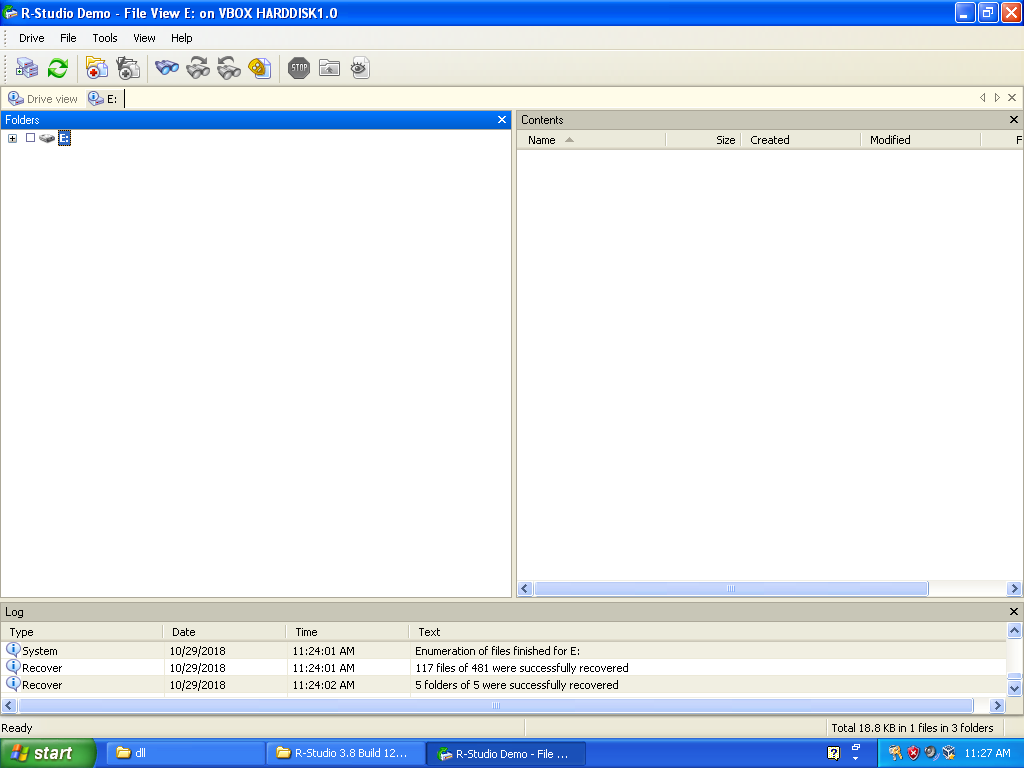
\includegraphics[height = 9\baselineskip]{./assets/y03s01-pcdiag-lab-03-p06.png}
		 		\caption{}
		 		\label{subfig:02-02-rstudio-res}
		 	\end{subfigure}
		 	\caption{Відновлення змісту тестової директорії програмою \textenglish{R-Studio}}
		 	\label{fig:02-rstudio-recovery}
		 \end{figure}

		\begin{figure}
			\centering
			\begin{subfigure}{0.5\columnwidth}
				\centering
				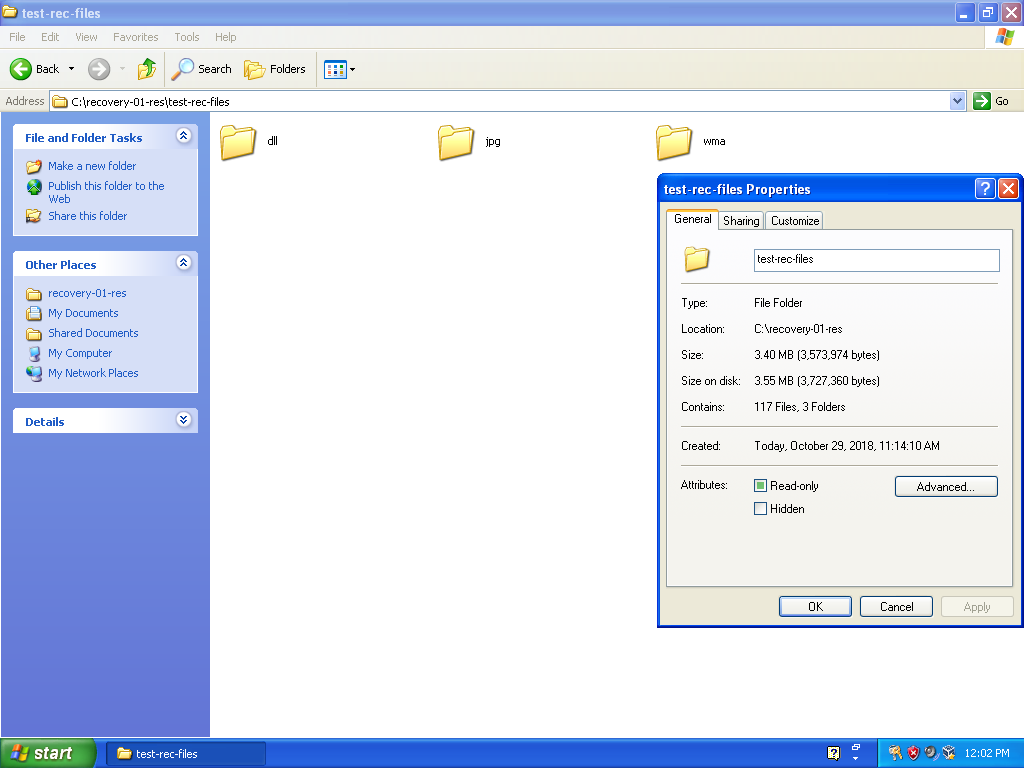
\includegraphics[height = 9\baselineskip]{./assets/y03s01-pcdiag-lab-03-p07.png}
				\caption{}
				\label{subfig:03-01-root}
			\end{subfigure}%
			\begin{subfigure}{0.5\columnwidth}
				\centering
				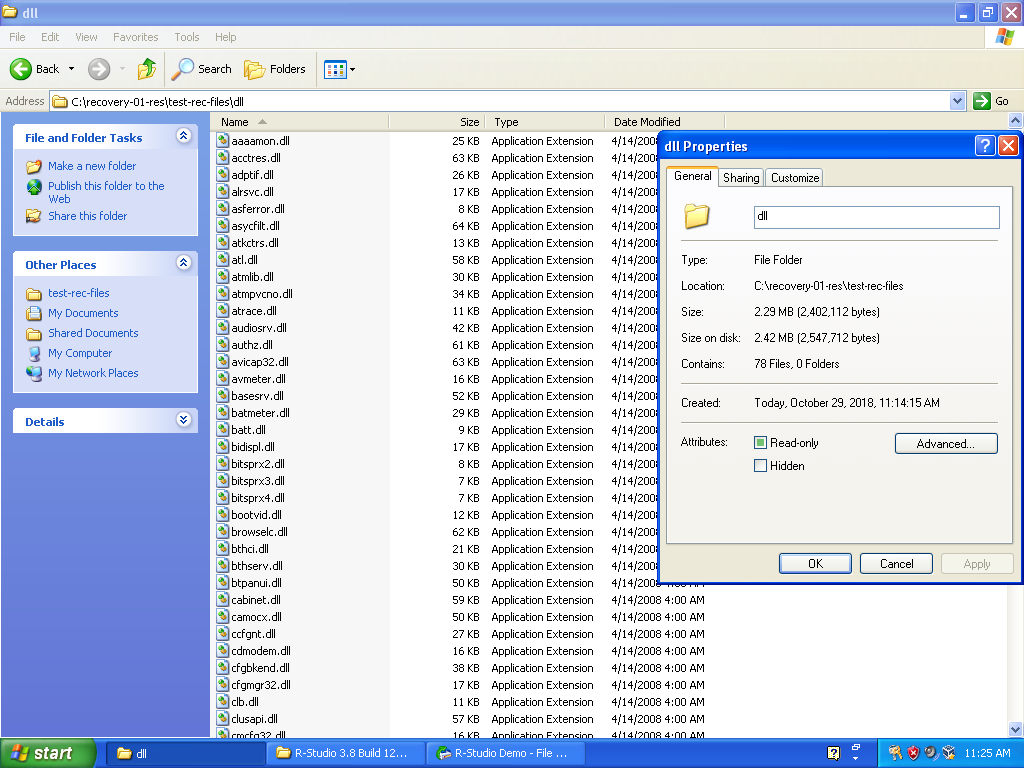
\includegraphics[height = 9\baselineskip]{./assets/y03s01-pcdiag-lab-03-p08.png}
				\caption{}
				\label{subfig:03-02-jpg}
			\end{subfigure}
			%
			\begin{subfigure}{0.5\columnwidth}
				\centering
				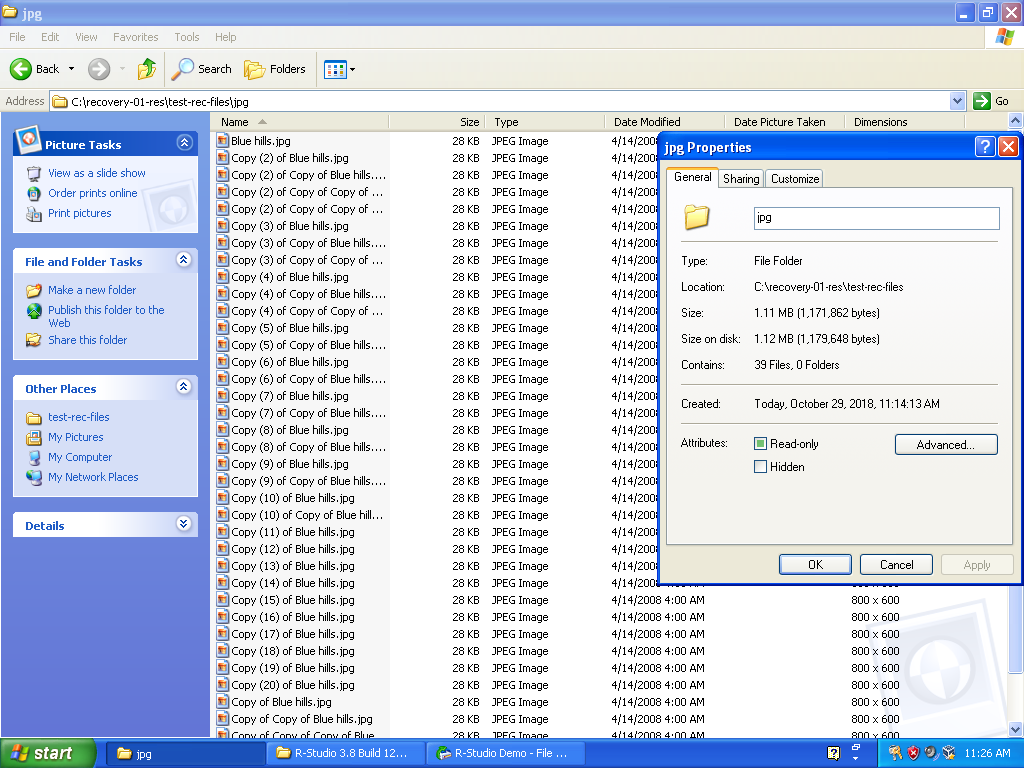
\includegraphics[height = 9\baselineskip]{./assets/y03s01-pcdiag-lab-03-p09.png}
				\caption{}
				\label{subfig:03-03-dll}
			\end{subfigure}%
			\begin{subfigure}{0.5\columnwidth}
				\centering
				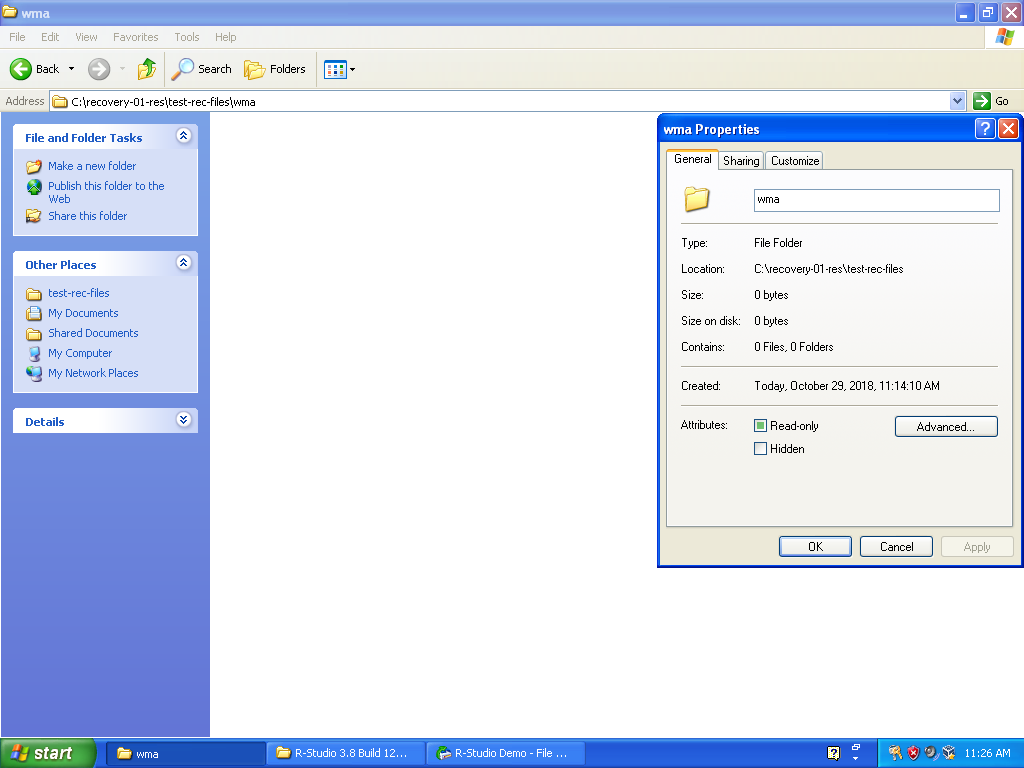
\includegraphics[height = 9\baselineskip]{./assets/y03s01-pcdiag-lab-03-p10.png}
				\caption{}
				\label{subfig:03-04-wav}
			\end{subfigure}%
			\caption{Директорії з даними, відновленими програмою~\textenglish{R-Studio}: \subref{subfig:03-01-root}~— корінь, \subref{subfig:03-02-jpg}–\subref{subfig:03-04-wav}~— за~типами файлів}
			\label{fig:03-rstudio-recovery-res}
		\end{figure}

		Створюємо нову тестову директорію, переміщуємо в~неї необхідні файли і~видаляємо їх. Запускаємо програму \textenglish{Zero Assumption Recovery}, обираємо директорію, зміст якої необхідно відновити, та~запускаємо процес~(рис.~\ref{fig:04-zar-recovery}). Після закінчення процесу відновлення отримали результат: з~479 початкових файлів програма знайшла та відновила 480~(рис.~\ref{fig:05-zar-recovery-res}).

		\begin{figure}[!htbp]
			\centering
			\begin{subfigure}{0.5\columnwidth}
				\centering
				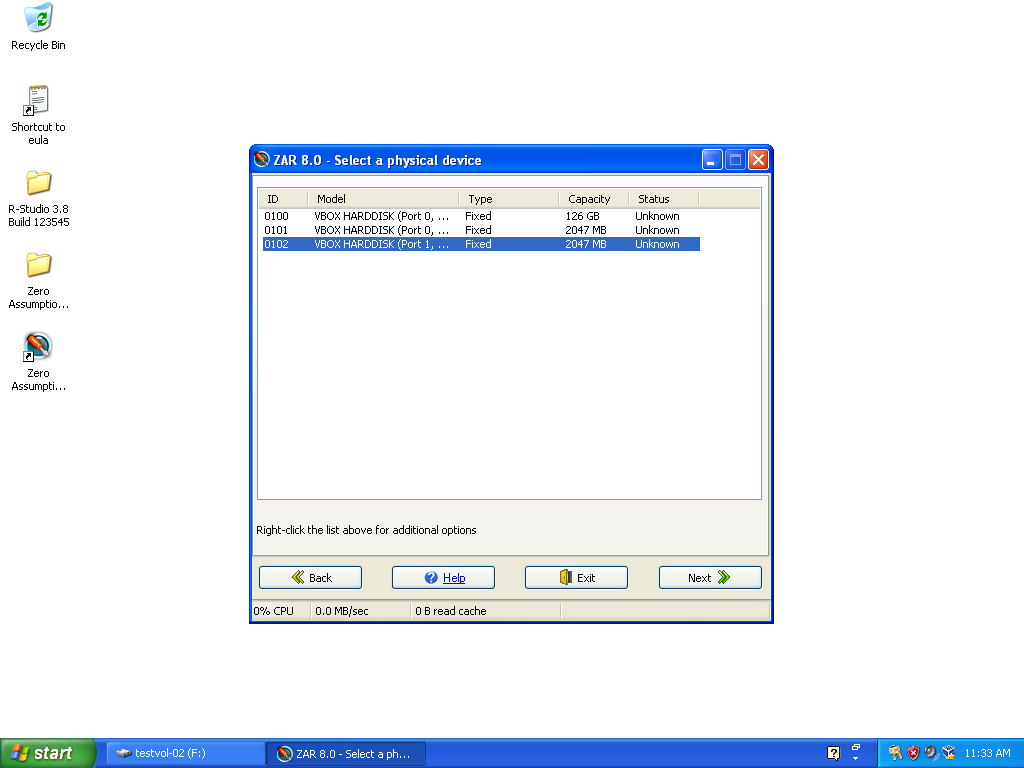
\includegraphics[height = 9\baselineskip]{./assets/y03s01-pcdiag-lab-03-p11.png}
				\caption{}
				\label{subfig:04-01-zar}
			\end{subfigure}%
			\begin{subfigure}{0.5\columnwidth}
				\centering
				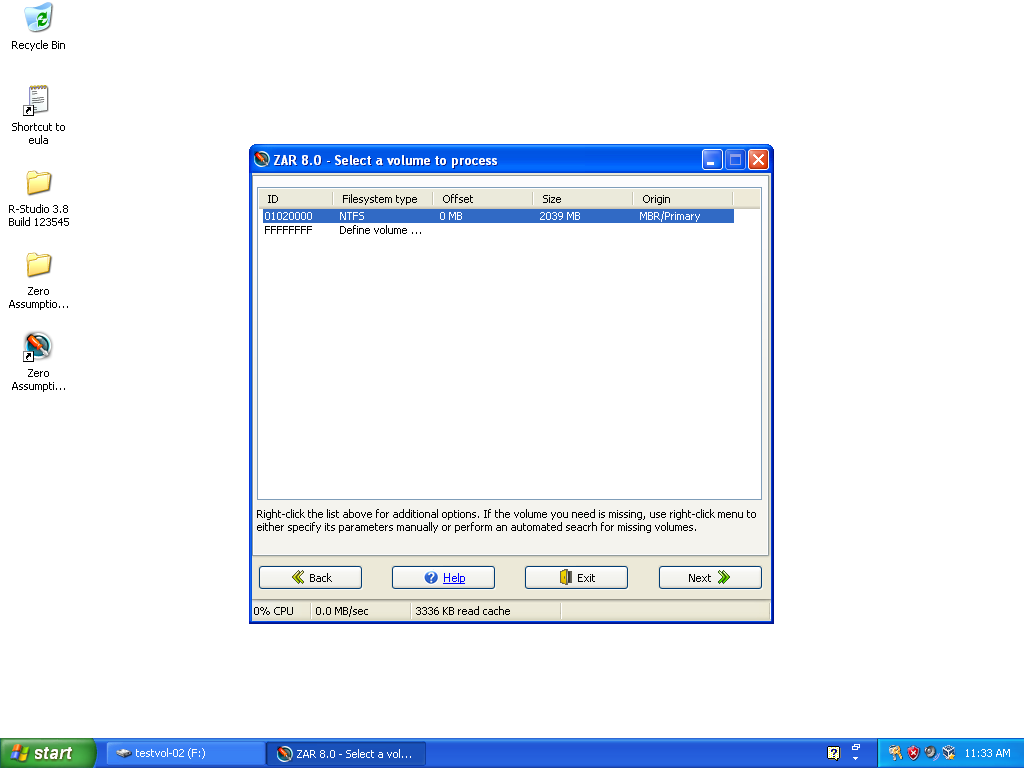
\includegraphics[height = 9\baselineskip]{./assets/y03s01-pcdiag-lab-03-p12.png}
				\caption{}
				\label{subfig:04-02-zar}
			\end{subfigure}
			%
			\begin{subfigure}{0.5\columnwidth}
				\centering
				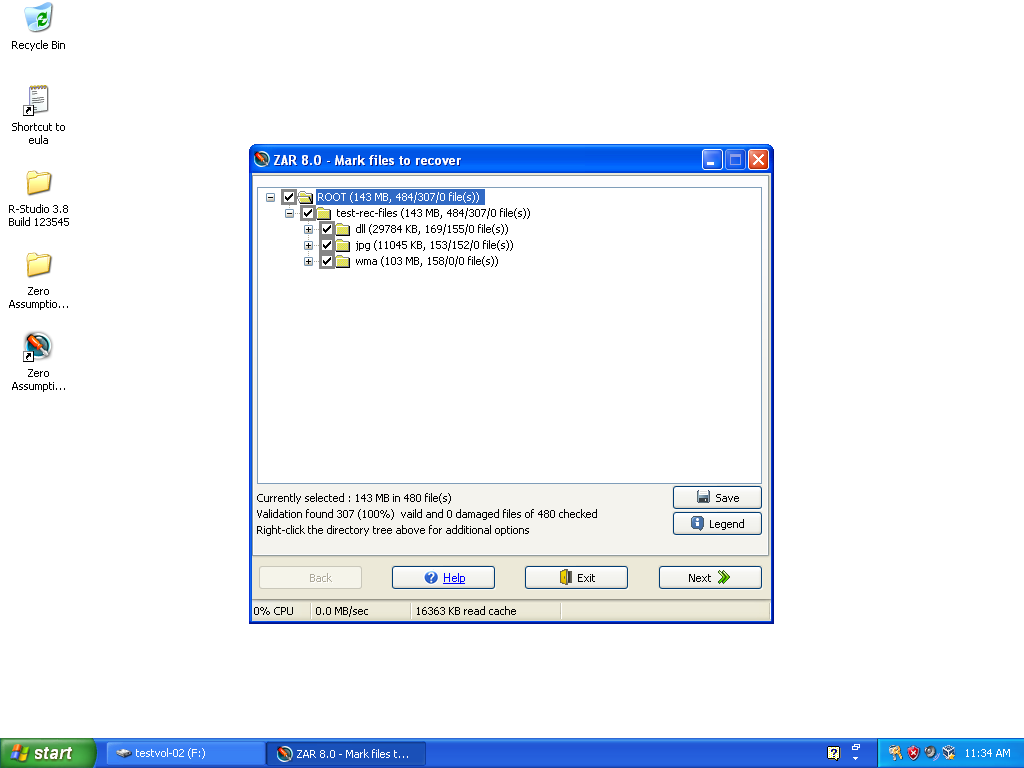
\includegraphics[height = 9\baselineskip]{./assets/y03s01-pcdiag-lab-03-p13.png}
				\caption{}
				\label{subfig:04-03-zar}
			\end{subfigure}%
			\begin{subfigure}{0.5\columnwidth}
				\centering
				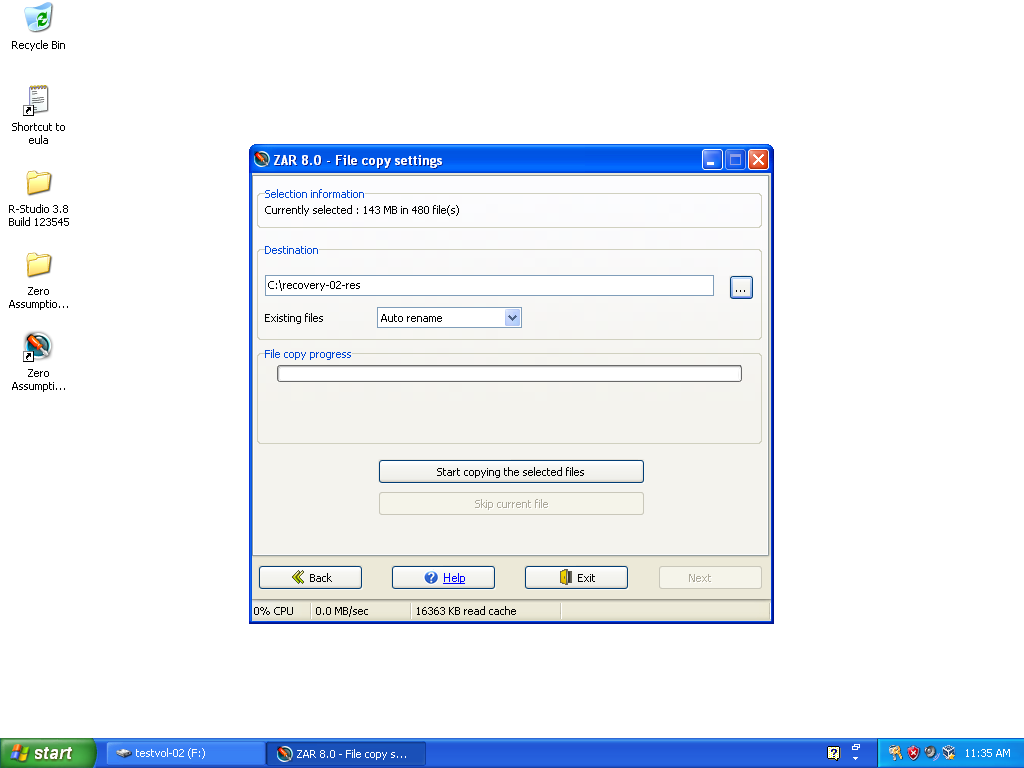
\includegraphics[height = 9\baselineskip]{./assets/y03s01-pcdiag-lab-03-p14.png}
				\caption{}
				\label{subfig:04-04-zar}
			\end{subfigure}
			\caption{Процес відновлення змісту тестової директорії програмою \textenglish{Zero Assumption Recovery}}
			\label{fig:04-zar-recovery}
		\end{figure}

		\begin{figure}
			\centering
			\begin{subfigure}{0.5\columnwidth}
				\centering
				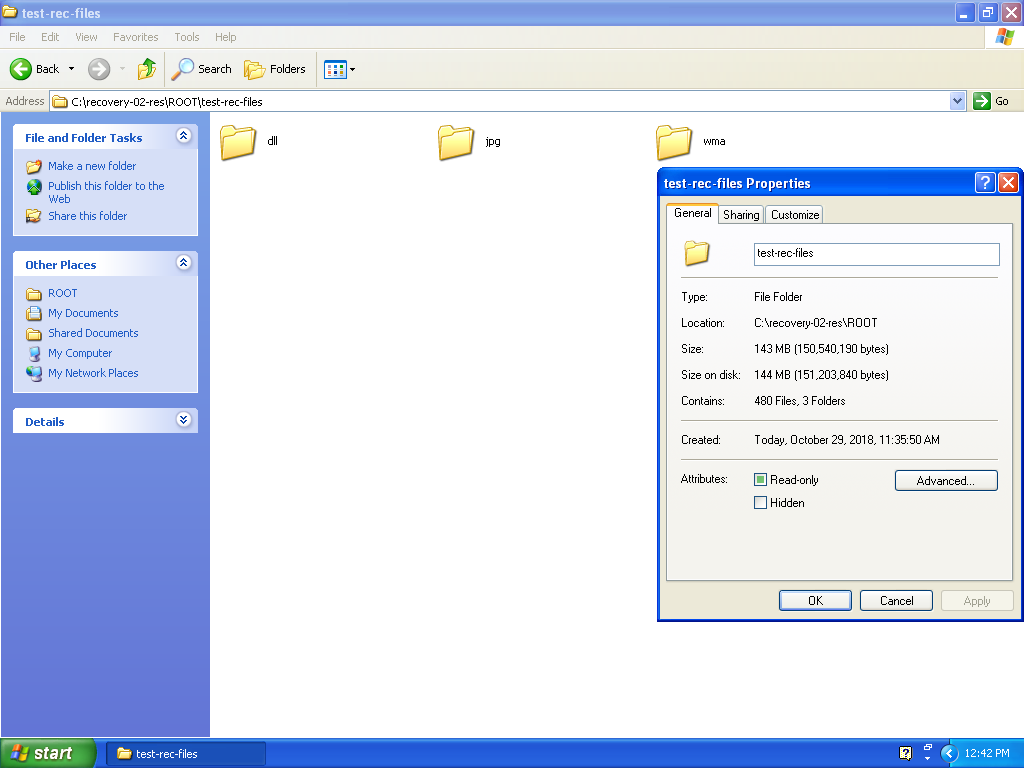
\includegraphics[height = 9\baselineskip]{./assets/y03s01-pcdiag-lab-03-p15.png}
				\caption{}
				\label{subfig:05-01-root}
			\end{subfigure}%
			\begin{subfigure}{0.5\columnwidth}
				\centering
				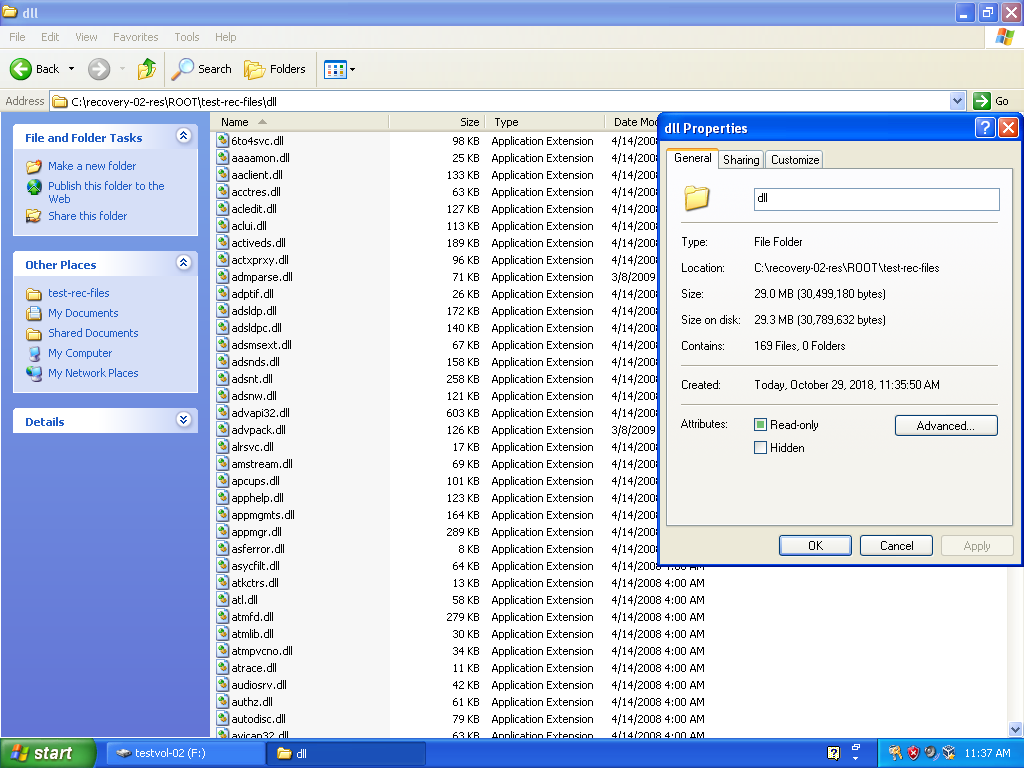
\includegraphics[height = 9\baselineskip]{./assets/y03s01-pcdiag-lab-03-p16.png}
				\caption{}
				\label{subfig:05-02-jpg}
			\end{subfigure}
			%
			\begin{subfigure}{0.5\columnwidth}
				\centering
				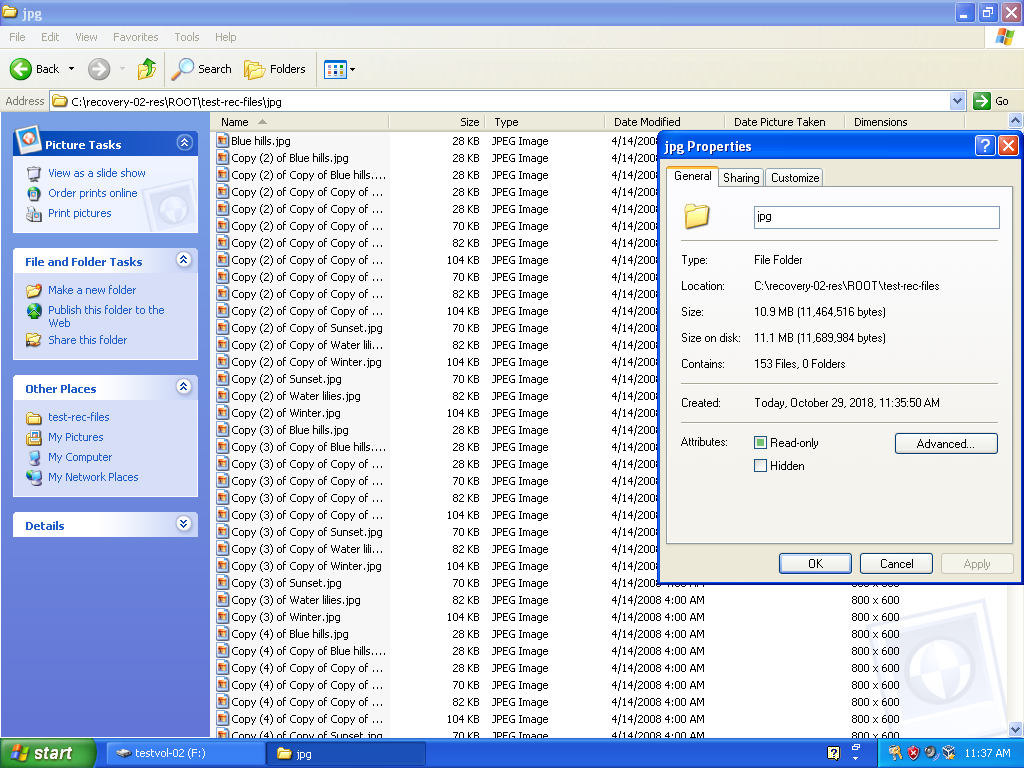
\includegraphics[height = 9\baselineskip]{./assets/y03s01-pcdiag-lab-03-p17.png}
				\caption{}
				\label{subfig:05-03-dll}
			\end{subfigure}%
			\begin{subfigure}{0.5\columnwidth}
				\centering
				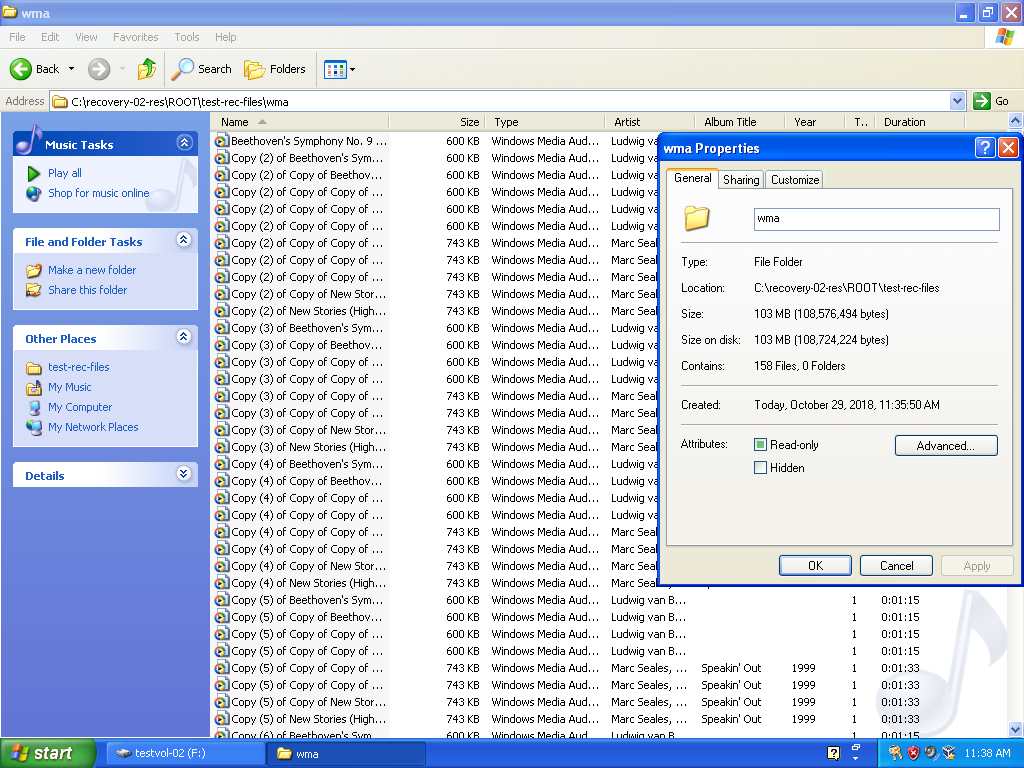
\includegraphics[height = 9\baselineskip]{./assets/y03s01-pcdiag-lab-03-p18.png}
				\caption{}
				\label{subfig:05-04-wav}
			\end{subfigure}%
			\caption{Директорії з даними, відновленими програмою~\textenglish{Zero Assumption Recovery}: \subref{subfig:05-01-root}~— корінь, \subref{subfig:05-02-jpg}–\subref{subfig:05-04-wav}~— за~типами файлів}
			\label{fig:05-zar-recovery-res}
		\end{figure}

	\section{Висновок}
		Виконуючи дану лабораторну роботу, ми~ознайомились з~методами відновлення даних на жорстких дисках на~прикладі програм \textenglish{R-Studio, Zero Assumption Recovery}. Програмі \textenglish{R-Studio} вдалось відновити 24\%~початкових файлів, коли \textenglish{Zero Assumption Recovery}~— на~1~файл більше початкового, тобто більше~100\%~(табл.~\ref{tab:01-recovery-details}). Це можна пояснити тим, що в процесі пошуку втрачених даних програма помилково знайшла заголовок вже знайденого файлу та відновила його як новий.

		\begin{table}[!htbp]
			\centering
			\caption{Результати відновлення даних: кількість файлів}
			\label{tab:01-recovery-details}
			\begin{tabular}{
					v{2\gridunitwidth - 2\tabcolsep}
					n{2\gridunitwidth - 2\tabcolsep}
					n{2\gridunitwidth - 2\tabcolsep}
					n{2\gridunitwidth - 2\tabcolsep}
					n{2\gridunitwidth - 2\tabcolsep}
					n{2\gridunitwidth - 2\tabcolsep}
			}
				\toprule
					 % & & \multicolumn{2}{c}{Кількість відновлених програмою файлів, шт.} \\
					 % & \multicolumn{5}{c}{Кількість файлів, шт.} \\
					 % \cmidrule(lr){2-6}
					 % & & \multicolumn{2}{c}{Відновлені програмою файли, шт.} \\
					 & До відновл. & \multicolumn{4}{r}{Після відновл. програмами} \\
					\cmidrule(lr){3-6}
					%Тип файлу & До відновлення, шт. & \textenglish{R-Studio} & \textenglish{ZAR} \\
					          &  & \multicolumn{2}{r}{\textenglish{R-Studio}} & \multicolumn{2}{r}{\textenglish{ZAR}} \\
					\cmidrule(lr){3-4} \cmidrule(lr){5-6}
					Тип файлу & шт. & шт. & \% & шт. & \%\\
				\midrule
					\textenglish{\allcaps{DLL}} & 169 &  78 & 46 & 169 & 100\\
					\textenglish{\allcaps{JPG}} & 152 &  39 & 26 & 153 & >100\\
					\textenglish{\allcaps{WMA}} & 158 &   0 & 0  & 158 & 100\\
					% \cmidrule(lr){1-3}
					Всього                      & 479 & 117 & 24 & 480 & >100 \\
					% З можливих                  & 000 & 1409 & 1409 \\
					% Відновлено, \%      &     &  24  & 100\\
				\bottomrule
			\end{tabular}
		\end{table}
\end{document}
